\documentclass[screen]{aomart}
\usepackage[T1]{fontenc}
\usepackage{lmodern}
\usepackage{amssymb,amsmath,graphicx,booktabs,listings,enumitem,xcolor,microtype}
\emergencystretch=2em
\setlength{\headheight}{14pt}
\copyrightnote{}
\doinumber{}
\pdfstringdefDisableCommands{\let\unskip\empty}
\hypersetup{colorlinks=true,linkcolor=blue!45!black,citecolor=blue!45!black,
  urlcolor=blue!45!black,pdftitle={Nilpotent-free spaces of 3 by 3 matrices over the field with three elements},pdfauthor={Deep Bhattacharjee}}
\newtheorem{theorem}{Theorem}[section]
\newtheorem{proposition}[theorem]{Proposition}
\newtheorem{lemma}[theorem]{Lemma}
\newtheorem{corollary}[theorem]{Corollary}
\newtheorem{conjecture}[theorem]{Conjecture}
\newtheorem*{theoremA}{Theorem A}
\newtheorem*{theoremB}{Theorem B}
\theoremstyle{definition}
\newtheorem{example}[theorem]{Example}
\newtheorem{question}[theorem]{Question}
\theoremstyle{remark}
\newtheorem{remark}[theorem]{Remark}
\numberwithin{equation}{section}
\newcommand{\F}{\mathbb{F}}
\newcommand{\M}{\mathrm{M}}
\newcommand{\sll}{\mathfrak{sl}}
\newcommand{\tr}{\operatorname{tr}}
\newcommand{\supp}{\operatorname{supp}}
\fancypagestyle{firstpage}{\fancyhf{}
  \fancyhead[C]{\scriptsize Manuscript prepared for submission, October 2026}
  \fancyfoot[C]{\footnotesize\thepage}}
\title[Nilpotent-free matrix spaces over F3]{\texorpdfstring{Nilpotent-free spaces of $3\times3$ matrices over the field with three elements}{Nilpotent-free spaces of 3 by 3 matrices over the field with three elements}}
\author{Deep Bhattacharjee}
\givenname{Deep}
\surname{Bhattacharjee}
\address{Formerly, Electro-Gravitational Space Propulsion Laboratory (EGSPL), Bhubaneswar, Odisha 751030, India}
\email{d.bhattacharjee@erl-forschung.de}
\email{itsdeep@live.com}
\urladdr{https://orcid.org/0000-0003-0466-750X}
\subject{primary}{msc2020}{15A30}
\subject{secondary}{msc2020}{15B33}
\subject{secondary}{msc2020}{11T99}
\keyword{nilpotent matrices}
\keyword{matrix spaces}
\keyword{finite fields}
\keyword{computer-assisted proof}
\thanks{Submission revision, 24 October 2026. Original preprint: \href{https://hexagonmath.org/2610.00480v1}{hexagon:2610.00480v1}. Revision DOI: \href{https://doi.org/10.5281/zenodo.23607867}{10.5281/zenodo.23607867}.}
\begin{document}
\begin{abstract}
We prove that the largest dimension of a linear subspace of the $3\times3$ matrices over the field with three elements whose only nilpotent element is zero is five. Thus the proposed existence, over every finite field, of a nilpotent-free space of dimension $n^2-\binom n2$ fails at $n=3$. An explicit five-dimensional example has a direct algebraic proof. For the upper bound, a complement to the strictly upper triangular matrices is the graph of a $3\times6$ coefficient matrix. A search tree covers all $3^{18}$ such matrices using $3{,}109{,}888$ nodes. We give the coverage proof and a complete independent C verifier. The accompanying Lean development formalizes the reduction and search soundness, with two compiled evaluations explicitly included in its trust base. We also describe the nilpotent cone in characteristic three as a quadric in a seven-dimensional quotient and give examples over the fields with two and five elements.
\end{abstract}
\maketitle
\section{Introduction}

Let $F$ be a field and $\M_n(F)$ the space of $n\times n$ matrices over $F$. Gerstenhaber~\cite{Ge} proved that a linear subspace of $\M_n(F)$ consisting of nilpotent matrices has dimension at most $\binom n2$ when $|F|\ge n$, and Serezhkin~\cite{Se} removed the condition on the field; de Seguins Pazzis extended the bound to division rings~\cite{dSP}. The strictly upper triangular matrices show that the bound is attained.

Wigderson~\cite{Wi} recently gave a proof by duality of Dieudonn\'e's theorem~\cite{Di,Me} that a space of singular $n\times n$ matrices has dimension at most $n^2-n$. Over a finite field the matrices of multiplication by the elements of $\F_{q^n}$ form an $n$-dimensional space in which every nonzero matrix is invertible, and a space of singular matrices meets it only in $0$; this gives the bound over finite fields, and a model-theoretic transfer carries it to every field. Wigderson proposed to treat the Gersten\-haber--\hspace{0pt}Serezhkin theorem in the same way. If $W\le\M_n(F)$ has dimension $n^2-\binom n2$ and no nonzero nilpotent element, then a space of nilpotent matrices of dimension larger than $\binom n2$ would meet $W$ in a nonzero matrix, which is impossible. Over $\mathbb R$ the symmetric matrices are such a space. For finite fields he made the following conjecture.

\begin{conjecture}[{Wigderson~\cite[Conjecture~8]{Wi}}]\label{conj:W}
For every finite field $F$ and every integer $n\ge1$ there is a linear subspace $W\le\M_n(F)$ with $\dim W=n^2-\binom n2$ such that no nonzero matrix in $W$ is nilpotent.
\end{conjecture}

We call a subspace \emph{nilpotent-free} if its only nilpotent element is $0$. For $n=3$ the conjecture asks for a nilpotent-free space of dimension six.

\begin{theoremA}
Every linear subspace of $\M_3(\F_3)$ of dimension at least six contains a nonzero nilpotent matrix. In particular Conjecture~\ref{conj:W} fails for $F=\F_3$ and $n=3$.
\end{theoremA}

\begin{theoremB}
The largest dimension of a nilpotent-free subspace of $\M_3(\F_3)$ is five. It is attained by
\begin{equation}\label{eq:W5}
W_5=\left\{\begin{pmatrix} a&0&b\\ 0&c-d-e&c\\ b&d&e\end{pmatrix} : a,b,c,d,e\in\F_3\right\}.
\end{equation}
\end{theoremB}

Theorem~A does not touch the Gersten\-haber--\hspace{0pt}Serezhkin theorem itself, which holds over every field. It shows that over $\F_3$ the bound for $3\times3$ matrices cannot be seen by exhibiting a single space, and it leaves the duality approach open over the algebraic closure of $\F_3$ (Remark~\ref{rem:transfer}).

The proof of Theorem~A reduces the statement to $3^{18}$ coefficient matrices (Section~\ref{sec:reduction}) and settles these by a search tree with $3{,}109{,}888$ nodes (Section~\ref{sec:tree}). The reduction, the soundness of the search and the deduction of both theorems are proved in the Lean~4 proof assistant~\cite{MU} with the Mathlib library~\cite{Mathlib}; the search itself is evaluated by compiled code inside Lean. Two exhaustive enumerations of a different kind, over all $678{,}468{,}820$ six-dimensional subspaces of $\M_3(\F_3)$ and over all $25{,}095{,}280$ five-dimensional subspaces of the trace-zero matrices, confirm Theorem~A independently.

The failure is special to the field. The conjecture holds for $n\le2$ over every finite field, and for $n=3$ over $\F_2$ and over $\F_5$ (Section~\ref{sec:holds}). In characteristic three the identity matrix has trace zero, and Section~\ref{sec:char3} shows how this shapes the nilpotent matrices in $\M_3$: they correspond one to one with the points of a quadric in the seven-dimensional quotient of the trace-zero matrices by the scalars, and no nilpotent-free space of dimension at least five contains the identity.

The original preprint is available at~\cite{Preprint}. The present submission revision, source files, independent verifier and verification records are available at~\cite{Revision}. The main upper bound uses an exhaustive computation. It does not assume any unproved statement from the preprint proposing the conjecture.

\section{Reduction to a finite statement}\label{sec:reduction}

Throughout, $E_{ij}$ denotes the matrix unit and $N_+=\langle E_{12},E_{13},E_{23}\rangle$ the space of strictly upper triangular $3\times 3$ matrices. We call
\[
p_1=(1,1),\ \ p_2=(2,2),\ \ p_3=(3,3),\ \ p_4=(2,1),\ \ p_5=(3,1),\ \ p_6=(3,2)
\]
the \emph{free positions}; they are the positions outside $N_+$. For a field $F$, a matrix $C\in F^{3\times6}$ and $y\in F^6$ put
\begin{equation}\label{eq:XC}
\begin{split}
X_C(y)&=\sum_{k=1}^{6}y_k E_{p_k}-(Cy)_1E_{12}-(Cy)_2E_{13}-(Cy)_3E_{23}\\
&=\begin{pmatrix} y_1&-(Cy)_1&-(Cy)_2\\ y_4&y_2&-(Cy)_3\\ y_5&y_6&y_3\end{pmatrix}.
\end{split}
\end{equation}
For $X\in\M_3(F)$ let $c_2(X)$ be the sum of the principal $2\times2$ minors, so that the characteristic polynomial of $X$ is $t^3-(\tr X)\,t^2+c_2(X)\,t-\det X$.

\begin{lemma}\label{lem:nil}
For $X\in\M_3(F)$ the following are equivalent: $X$ is nilpotent; $X^3=0$; $\tr X=c_2(X)=\det X=0$.
\end{lemma}

\begin{proof}
A nilpotent matrix has only the eigenvalue $0$ over an algebraic closure of $F$, so its characteristic polynomial is $t^3$; this is the third condition. By the Cayley--Hamilton theorem the third condition gives $X^3=0$, which in turn means that $X$ is nilpotent.
\end{proof}

\begin{lemma}\label{lem:graph}
Let $W\le\M_3(F)$ with $\dim W\ge6$. Then $W\cap N_+\ne0$, or $\dim W=6$ and there is a unique $C\in F^{3\times6}$ with $W=\{X_C(y):y\in F^6\}$.
\end{lemma}

\begin{proof}
Suppose $W\cap N_+=0$. Then $\dim W\le 9-\dim N_+=6$, so $\dim W=6$ and $\M_3(F)=W\oplus N_+$. The map $\pi\colon\M_3(F)\to F^6$, $X\mapsto (X_{p_1},\dots,X_{p_6})$, has kernel $N_+$, so its restriction to $W$ is an isomorphism. For $y\in F^6$ the upper entries $(X_{12},X_{13},X_{23})$ of $X=(\pi|_W)^{-1}(y)$ depend linearly on $y$; writing them as $-Cy$ defines $C$, and then $X=X_C(y)$. Uniqueness is clear.
\end{proof}

\begin{proposition}\label{prop:finite}
For every $C\in\F_3^{3\times6}$ there is a nonzero $y\in\F_3^6$ with $X_C(y)^3=0$.
\end{proposition}

The proof of Proposition~\ref{prop:finite} occupies Section~\ref{sec:tree}. We first derive the two theorems from it.

\begin{proof}[Proof of Theorem~A]
Let $W\le\M_3(\F_3)$ have dimension at least six, and let $W'\le W$ be a subspace of dimension exactly six. A nonzero element of $W'\cap N_+$ is a nonzero nilpotent element of $W$. Otherwise, by Lemma~\ref{lem:graph}, $W'=\{X_C(y)\}$ for some $C$, and Proposition~\ref{prop:finite} gives $y\ne0$ with $X_C(y)^3=0$. The matrix $X_C(y)$ is nilpotent by Lemma~\ref{lem:nil}, and nonzero because its entries at the free positions are $y$.
\end{proof}

\begin{proof}[Proof of Theorem~B]
The five parameters of~\eqref{eq:W5} appear alone in the entries $(1,1)$, $(1,3)$, $(2,3)$, $(3,2)$ and $(3,3)$, so $\dim W_5=5$. We prove nilpotent-freeness directly. Suppose $X\in W_5$ is nilpotent and put $p=c-d$ and $z=c+d$. The equation $\tr X=0$ gives $a=-p$. Expanding the principal minors, and then simplifying the determinant using $c_2(X)=0$, gives
\[
0=c_2(X)=-z^2+pe-e^2-b^2,\qquad
0=\det X=-p+(p+e)b^2.
\]
Here $p^3=p$ in $\F_3$. If $b=0$, the second equation gives $p=0$, and the first gives $z^2+e^2=0$. Each square in $\F_3$ is $0$ or $1$, so $z=e=0$. Since $c-d=c+d=0$ and $2\ne0$, also $c=d=0$, and then $a=0$. If $b\ne0$, then $b^2=1$ and the determinant equation gives $e=0$. The first equation would give $z^2=-1=2$, which is impossible in $\F_3$. Thus $X=0$. This proves the lower bound without a finite enumeration; Theorem~A proves the upper bound.
\end{proof}

\section{The search tree}\label{sec:tree}

\subsection{Partial matrices}
The columns of $C$ correspond to the free positions, column $k$ to $p_k$. We fix them one at a time in the order
\begin{equation}\label{eq:order}
\sigma=(\sigma_1,\dots,\sigma_6)=(4,5,6,1,2,3),
\end{equation}
that is, first the three strictly lower positions $(2,1)$, $(3,1)$, $(3,2)$ and then the diagonal (Figure~\ref{fig:board}). Let $S_d=\{\sigma_1,\dots,\sigma_d\}$. A \emph{node of depth $d$} is an assignment of values in $\F_3^3$ to the columns $\sigma_1,\dots,\sigma_d$; it is \emph{extended} by every $C$ whose columns in $S_d$ take these values.

\begin{figure}[ht]
\centering
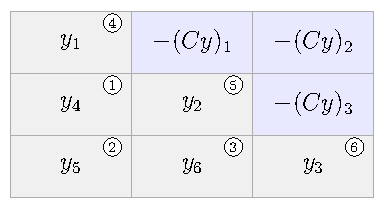
\includegraphics[width=0.66\textwidth]{figures/board.pdf}
\caption{The matrix $X_C(y)$ of~\eqref{eq:XC}. The six free positions carry the coordinates of $y$; the three raised positions carry $-Cy$. The circled numbers give the order~\eqref{eq:order} in which the corresponding columns of $C$ are fixed: the strictly lower positions first, then the diagonal.}
\label{fig:board}
\end{figure}

The search rests on a locality property. If $\supp y\subseteq S_d$, then $Cy=\sum_{k\in S_d}y_k\,C_{\ast k}$ involves only the columns of $C$ in $S_d$, so $X_C(y)$ is the same matrix for every $C$ extending a given node. We call a node of depth $d\ge1$ \emph{closed} if there is $y\in\F_3^6$ with $\supp y\subseteq S_d$, $y_{\sigma_d}=1$ and $X_C(y)^3=0$, for $C$ extending the node; by locality such a $y$ serves every extension at once.\footnote{Restricting to $y_{\sigma_d}=1$ loses nothing. A vector $y\ne0$ with support in $S_d$ has a largest $e\le d$ with $y_{\sigma_e}\ne0$; after multiplying by $\pm1$, which does not affect nilpotency, $y_{\sigma_e}=1$, and $y$ is a candidate at the ancestor of depth $e$.}

The tree is built from the root, the unique node of depth $0$: a node of depth $d<6$ that is not closed receives as children its $27$ extensions to depth $d+1$. Proposition~\ref{prop:finite} follows once every node of depth $6$ in this tree is closed. Indeed, given $C$, consider the nodes on the path from the root to the node of depth $6$ that $C$ determines; the first closed node on the path exists and lies in the tree, and its witness $y$ gives $X_C(y)^3=0$.

\begin{proposition}\label{prop:tree}
The tree has $3{,}109{,}888$ nodes, and every node of depth $6$ is closed. A complete executable verifier using characteristic-polynomial coefficients is printed in Appendix~\ref{app:verifier}. Table~\ref{tab:tree} gives the counts by depth.
\end{proposition}

\begin{table}[ht]
\centering
\begin{tabular}{@{}rrrr@{}}
\toprule
Depth $d$ & Nodes & Closed nodes & Open nodes\\
\midrule
0 & 1 & 0 & 1\\
1 & 27 & 9 & 18\\
2 & 486 & 228 & 258\\
3 & 6,966 & 5,165 & 1,801\\
4 & 48,627 & 0 & 48,627\\
5 & 1,312,929 & 1,248,453 & 64,476\\
6 & 1,740,852 & 1,740,852 & 0\\
\bottomrule
\end{tabular}
\medskip
\caption{The search tree of Proposition~\ref{prop:tree}. Each open node of depth $d<6$ has $27$ children.}
\label{tab:tree}
\end{table}



The shape of the tree has a simple explanation. While only lower columns are fixed ($d\le3$), the candidates $y$ are supported on the strictly lower positions, so $X_C(y)$ has zero diagonal and is nilpotent exactly when $c_2(X_C(y))=\det X_C(y)=0$; already three quarters of the nodes of depth $3$ close in this way. At depth $4$ the candidates have $y_1=1$ and no other diagonal entry, hence trace $1$, and no node closes. At depths $5$ and $6$ the trace condition can be met, and the remaining nodes close.

\subsection{Formal verification}\label{sec:lean}
The search tree, the soundness argument and the reduction of Section~\ref{sec:reduction} are formalised in Lean~4~\cite{MU} with Mathlib~\cite{Mathlib}; the development is archived with this paper~\cite{Ar}. It consists of three parts.
\begin{enumerate}[label=(\roman*),leftmargin=*]
\item A search function written in plain Lean, without Mathlib, which explores the tree above with the cube test of Lemma~\ref{lem:nil} written out entry by entry, together with a check that every candidate vector at depth $d$ is nonzero and supported on $S_d$.
\item A proof, by induction on the number of columns still to be fixed, that if the search function and the candidate check both return \emph{true}, then Proposition~\ref{prop:finite} holds.
\item A proof of Lemma~\ref{lem:graph} for subspaces in Mathlib's sense, with dimension given by \emph{finrank}, from which Theorem~A, the negation of Conjecture~\ref{conj:W} as a formal statement over all finite fields, and Theorem~B follow.
\end{enumerate}
The two Boolean equations of part (i) are evaluated by compiled code; this takes about four and a half minutes on one core. Lean records each such evaluation as an axiom asserting exactly the evaluated equation, so the trusted base consists of the Lean kernel, the three standard axioms (propositional extensionality, choice and soundness of quotients), and the Lean compiler for these two equations. The archived check of the $242$ nonzero matrices of $W_5$ is done by the kernel; the proof of Theorem~B above now gives a separate algebraic argument.

The development also contains Lemma~\ref{lem:shift}, the two statements of Lemma~\ref{lem:quadric} used later (the formula for $c_2$ and the fact that the radical is $FI$), Propositions~\ref{prop:cone} and~\ref{prop:identity} (the latter with Mathlib's Chevalley--Warning theorem), Proposition~\ref{prop:two} for every finite field, and Examples~\ref{ex:F2} and~\ref{ex:F5}, whose finite checks are again done by the kernel. These use only the three standard axioms. The elementary proof of the quadric zero count in Lemma~\ref{lem:finitequadric}, the revised algebraic proof of Theorem~B, and the independent C verifier in Appendix~\ref{app:verifier} are written proofs or computations separate from this formalisation. No additional formal-verification claim is made for these revisions.

\subsection{Independent computations}
The preceding archive reports two exhaustive enumerations of a different kind. The trace-zero enumeration was independently rerun on 24 October 2026; the larger enumeration and the full nilpotent-line histogram were not rerun for this submission revision and are supplementary to the proof in Appendix~\ref{app:verifier}.

First, a six-dimensional subspace $W\le\M_3(\F_3)$ is the orthogonal complement $U^\perp$ of a three-dimensional $U\le\F_3^9$ for the standard dot product on matrix entries, and $U$ is the row space of a unique $3\times9$ matrix in reduced row echelon form. The subspace $W$ is nilpotent-free exactly when each of the $364$ lines of nonzero nilpotent matrices is not orthogonal to $U$. Running through all $\binom{9}{3}_3=678{,}468{,}820$ echelon matrices, no nilpotent-free $W$ occurs. (That there are $364=(3^6-1)/2$ such lines is the theorem of Fine and Herstein~\cite{FH} that $\M_n(\F_q)$ contains exactly $q^{n^2-n}$ nilpotent matrices.)

Second, if $\dim W=6$ then $W\cap\sll_3(\F_3)$ has dimension at least five, where $\sll_3$ denotes the trace-zero matrices. All $\binom 83_3=25{,}095{,}280$ five-dimensional subspaces of $\sll_3(\F_3)$ contain a nonzero nilpotent matrix, which is a second proof of Theorem~A that does not use Lemma~\ref{lem:graph}. The search tree has also been written again in C++, with the same node counts. The programs are archived with the paper~\cite{Ar}.

\section{Characteristic three}\label{sec:char3}

In this section $F=\F_q$ with $q=3^k$. Since $\tr I=3=0$, the identity lies in $\sll_3(F)$.

\begin{lemma}\label{lem:shift}
For $X\in\sll_3(F)$ and $a\in F$,
\[
c_2(X+aI)=c_2(X),\qquad \det(X+aI)=\det X+a^3+a\,c_2(X).
\]
\end{lemma}

\begin{proof}
The characteristic polynomial of $X$ is $\chi(t)=t^3+c_2(X)\,t-\det X$. In characteristic three $(t-a)^3=t^3-a^3$, so the characteristic polynomial of $X+aI$ is
\[
\chi(t-a)=t^3+c_2(X)\,t-\bigl(\det X+a^3+a\,c_2(X)\bigr),
\]
and the two identities can be read off.
\end{proof}

\begin{lemma}\label{lem:quadric}
On $\sll_3(F)$ one has $c_2(X)=\tr(X^2)$. The polar form of $c_2$ is $(X,Y)\mapsto 2\tr(XY)$, whose radical in $\sll_3(F)$ is the line $FI$. Hence $c_2$ induces a nondegenerate quadratic form $\bar c_2$ on the seven-dimensional space $V=\sll_3(F)/FI$.
\end{lemma}

\begin{proof}
Newton's identity $2c_2(X)=(\tr X)^2-\tr(X^2)$ gives $c_2(X)=-\tfrac12\tr(X^2)=\tr(X^2)$ on $\sll_3(F)$, because $-\tfrac12=1$ in $F$. The polar form is $c_2(X+Y)-c_2(X)-c_2(Y)=2\tr(XY)$. The trace form is nondegenerate on $\M_3(F)$, and the orthogonal complement of $\sll_3(F)=(FI)^\perp$ is $FI$; since $FI\subseteq\sll_3(F)$, the radical of the restriction to $\sll_3(F)$ is $FI$. The form is constant on cosets of $FI$ by Lemma~\ref{lem:shift}, and as $q$ is odd it is nondegenerate on the quotient.
\end{proof}

\begin{lemma}\label{lem:finitequadric}
Let $F=\F_q$ have odd cardinality. Every quadratic form on $F^m$, $m\ge3$, has a nonzero zero. A nondegenerate quadratic form in seven variables has exactly $q^6$ zeros, including zero.
\end{lemma}
\begin{proof}
Diagonalise the form. If it is degenerate, a nonzero vector of its radical is a zero. Otherwise choose three diagonal coefficients $a,b,c\ne0$. The sets $\{ax^2:x\in F\}$ and $\{-c-by^2:y\in F\}$ each have $(q+1)/2$ elements, so they intersect. Their intersection gives $ax^2+by^2+c=0$, a nonzero zero with third coordinate $1$.

A nondegenerate form in dimension at least three therefore has an isotropic vector and splits off a hyperbolic plane. Explicitly, for an isotropic $v\ne0$ choose $w$ with polar pairing $B(v,w)=1$ and replace it by $w-Q(w)v$; both vectors are isotropic and their span is nondegenerate, with form $xy$. Repeating, a seven-dimensional form is the orthogonal sum of three such planes and a nonzero one-dimensional form. If $N_m$ is the number of zeros before adjoining one plane, then
\[
 N_{m+2}=(2q-1)N_m+(q-1)(q^m-N_m)
        =qN_m+(q-1)q^m,
\]
because $xy=0$ has $2q-1$ solutions and $xy=t\ne0$ has $q-1$. Starting from $N_1=1$ gives $N_3=q^2$, $N_5=q^4$ and $N_7=q^6$.
\end{proof}

\begin{proposition}\label{prop:cone}
The quotient map $\sll_3(F)\to V$ restricts to a bijection from the set of nilpotent matrices in $\M_3(F)$ onto the set of zeros of $\bar c_2$.
\end{proposition}

\begin{proof}
A nilpotent matrix lies in $\sll_3(F)$ and has $c_2=0$ by Lemma~\ref{lem:nil}, so it maps to a zero of $\bar c_2$. Conversely let $X\in\sll_3(F)$ with $c_2(X)=0$. By Lemmas~\ref{lem:nil} and~\ref{lem:shift}, $X+aI$ is nilpotent exactly when $\det X+a^3=0$. The map $a\mapsto a^3$ is the Frobenius automorphism of $F$, so there is exactly one such $a$.
\end{proof}

By Lemma~\ref{lem:finitequadric}, a nondegenerate quadratic form in seven variables over $\F_q$ has exactly $q^6$ zeros, so Proposition~\ref{prop:cone} gives a short proof, for $n=3$ and $q$ a power of three, of the count $q^{n^2-n}$ of Fine and Herstein.

\begin{proposition}\label{prop:identity}
Let $U\le\sll_3(F)$ with $I\in U$ and $\dim U\ge4$. Then $U$ contains a nonzero nilpotent matrix. Consequently a nilpotent-free subspace of $\M_3(F)$ of dimension at least five does not contain $I$.
\end{proposition}

\begin{proof}
The image of $U$ in $V$ has dimension at least three, and the restriction of $\bar c_2$ to it is a quadratic form in at least three variables, which has a nonzero zero by Lemma~\ref{lem:finitequadric}. Choose $X\in U\setminus FI$ mapping to it. By Proposition~\ref{prop:cone} some $X+aI$ is nilpotent; it lies in $U$ because $I\in U$, and it is nonzero because $X\notin FI$. For the second statement, if $W$ is nilpotent-free with $\dim W\ge5$ and $I\in W$, apply the first to $U=W\cap\sll_3(F)$, which contains $I$ and has dimension at least $\dim W-1\ge4$.
\end{proof}

By Proposition~\ref{prop:identity}, the second computation of Section~\ref{sec:tree} need only consider five-dimensional subspaces $U\le\sll_3(\F_3)$ with $I\notin U$. For such $U$ the space $U\oplus FI$ maps onto a five-dimensional subspace $\bar U$ of $V$, every zero of $\bar c_2$ on $\bar U$ has exactly one nilpotent lift in $U\oplus FI$, and the question is whether one of these lifts lies in the hyperplane $U$. A nondegenerate form on $\bar U$ has $40$ projective zeros, and each lift lies in $U$ with a chance of one in three if the lifts behave independently. The archived enumeration agrees with this heuristic on average, the mean number of nilpotent lines being close to $40/3$, and shows how little room there is at the extreme: $1{,}872$ of the five-dimensional subspaces of $\sll_3(\F_3)$ contain exactly one line of nilpotent matrices. These average counts do not by themselves prove Theorem~A, and we do not know a proof of its upper bound that avoids the computation.

\section{Fields where the conjecture holds}\label{sec:holds}

\begin{proposition}\label{prop:two}
Conjecture~\ref{conj:W} holds for $n\le2$ and every finite field $F$.
\end{proposition}

\begin{proof}
For $n=1$ take $W=F$. For $n=2$ choose $M\in\M_2(F)$ such that the binary quadratic form $u\mapsto u^{\mathsf T}Mu$ has no nonzero zero; such forms exist over every finite field, for instance the norm form of $\F_{q^2}$ over $F$ written in a basis. Let $J=\left(\begin{smallmatrix}0&-1\\1&0\end{smallmatrix}\right)$ and $W=\{X:\tr(JMX)=0\}$, a space of dimension $3=2^2-\binom22$. A nonzero nilpotent $X\in\M_2(F)$ has rank one and square zero, so $X=uv^{\mathsf T}$ with $u,v\ne0$ and $v^{\mathsf T}u=0$, that is $v=\lambda Ju$ with $\lambda\ne0$. Then $\tr(JMX)=v^{\mathsf T}JMu=\lambda\,u^{\mathsf T}J^{\mathsf T}JMu=\lambda\,u^{\mathsf T}Mu\ne0$, so $X\notin W$.
\end{proof}

\begin{example}\label{ex:F2}
Over $\F_2$ the space
\[
\left\{\begin{pmatrix} a&b+d+e&a+e+f\\ d&b&b+f\\ e&f&c\end{pmatrix} : a,\dots,f\in\F_2\right\}
\]
is six-dimensional and nilpotent-free, so the conjecture holds for $n=3$ over $\F_2$. By Lemma~\ref{lem:graph} a nilpotent-free six-dimensional subspace is $\{X_C(y)\}$ for a unique $C$, and running through the $2^{18}$ matrices $C\in\F_2^{3\times6}$ shows that exactly $128$ of the $\binom93_2=788{,}035$ six-dimensional subspaces of $\M_3(\F_2)$ are nilpotent-free.
\end{example}

\begin{example}\label{ex:F5}
Over $\F_5$ the space of matrices
\[
\begin{pmatrix} a&3a+4b+d+2e+2f&3a+3b+3e+3f\\ d&b&a+4b+c+3d+3f\\ e&f&c\end{pmatrix},\qquad a,\dots,f\in\F_5,
\]
is six-dimensional and nilpotent-free, as a check of its $5^6-1$ nonzero elements shows. So the conjecture holds for $n=3$ over $\F_5$.
\end{example}

For $q\in\{4,7,8,9\}$ we do not know whether $\M_3(\F_q)$ has a nilpotent-free subspace of dimension six. By Lemma~\ref{lem:graph} such a subspace is $\{X_C(y)\}$ for some $C\in\F_q^{3\times6}$, and a local search over $C$, which found the examples over $\F_2$ and $\F_5$, found none for these fields in twenty-five minutes each. We draw no conclusion from this.

\section{Remarks and questions}\label{sec:questions}

\begin{remark}\label{rem:transfer}
Theorem~A does not rule out a duality proof of the Gersten\-haber--\hspace{0pt}Serezhkin bound over $\overline{\F}_3$. A space $N$ of nilpotent matrices over $\overline{\F}_3$ is spanned by finitely many matrices, whose entries lie in some $\F_{3^k}$; their span over $\F_{3^m}$ for any multiple $m$ of $k$ consists of nilpotent matrices and has the same dimension as $N$. It therefore suffices to have nilpotent-free spaces of dimension $n^2-\binom n2$ over $\F_{3^m}$ for some multiple $m$ of every $k$. Theorem~A only removes $m=1$.
\end{remark}

\begin{question}
Does $\M_3(\F_9)$ contain a nilpotent-free subspace of dimension six? More generally, for which $n$ and $q$ is the largest dimension of a nilpotent-free subspace of $\M_n(\F_q)$ smaller than $n^2-\binom n2$?
\end{question}

Proposition~\ref{prop:identity} holds over every finite field of characteristic three, and a similar but weaker phenomenon is available whenever the characteristic divides $n$, since then $I\in\sll_n$. It would be interesting to know whether the conjecture fails for other pairs $(n,q)$ with $p\mid n$, or whether $(3,\F_3)$ is an isolated exception.

\appendix
\section{Executable finite verification}\label{app:verifier}
The following self-contained C program verifies Proposition~\ref{prop:tree}. Compile it, for example, with \texttt{cc -O3 -std=c11 audit\_tree.c -o audit\_tree} and run \texttt{./audit\_tree}. It has no input and uses no random choices. Its successful run reproduces Table~\ref{tab:tree} and exits with status zero only when the table, the recurrence ``children $=27\times$ open parents'', and the absence of open leaves all agree. The table comparison is a consistency check: the exhaustive recursion and the witness test supply the mathematical verification.

The variable \texttt{coef} is $C$. Each witness has value $1$ at the newest fixed column and is zero at all unfixed columns, hence is nonzero and depends on no later assignment. The test uses $\tr X=c_2(X)=\det X=0$ from Lemma~\ref{lem:nil}, independently of the matrix-cube implementation used in the Lean search. All products and sums are of small integers and the counters are 64-bit unsigned integers, so no overflow occurs. Depth is at most six. Every possible next column occurs in the loop from $0$ to $26$. Induction on the remaining depth, as in Section~\ref{sec:tree}, proves coverage of all $3^{18}$ coefficient matrices.

The independent verifier printed here visits $3{,}109{,}888$ nodes and leaves no open leaf. A separate rerun of the archived trace-zero enumeration checks $25{,}095{,}280$ subspaces and also finds none without a nonzero nilpotent. These are exhaustive computations, not numerical evidence from a sample. As with other computer-assisted proofs, correctness of the compiler and execution environment is part of the computational trust base; compilation alone is not the result of the check.

\lstinputlisting[basicstyle=\ttfamily\scriptsize,breaklines=true,columns=fullflexible,keepspaces=true,frame=single,language=C]{audit_tree.c}


\section*{Reproducibility}
The complete submission source, pinned Lean development, independent C verifier and verification records are available at~\cite{Revision}. The preceding archive is~\cite{Ar}. Section~\ref{sec:lean} identifies precisely which statements are formalized and which checks use compiled evaluation. The code in Appendix~\ref{app:verifier} is sufficient for the exhaustive upper bound; the two larger enumerations are independent supplements.

\section*{Use of generative AI}
Claude (Anthropic) assisted the original searches, computations, Lean development and drafting. OpenAI Codex assisted the direct algebraic proof of the five-dimensional construction in the proof of Theorem~B in Section~\ref{sec:reduction}; the elementary quadratic-form argument in Lemma~\ref{lem:finitequadric}; and the independently written characteristic-coefficient verifier in Appendix~\ref{app:verifier}. It also assisted proof auditing, scope corrections, exact checks, bibliography and typesetting. The human author is responsible for reviewing and approving the mathematical content and the accuracy of the citations.

\bibliographystyle{aomplain}
\bibliography{references}
\end{document}
